\scanpage{40}
\mspage{\handwritten{8}}
% archive sheet number: 39
est défini comme en (7.2 (vii)). Nous pouvons définir, par les mêmes formules qu'en (7.2 (vii)et 7.1 (ii)), les morphismes $\handwritten{\unsure{\gamma|\upsilon}}':A'\handwritten{\times}_{S'}B'\handwritten{\longrightarrow}G'$ et $\handwritten{\unsure{\gamma|\upsilon}}'^n:(A'\handwritten{\times}_{S'}B')^n\handwritten{\longrightarrow}G'$, on a bien $\handwritten{\unsure{\gamma|\upsilon}}'^n_{(\handwritten{\kappa}(\handwritten{\eta}))}=\handwritten{\unsure{\gamma|\upsilon}}^n_{\handwritten{\eta}}$. Par conséquent (EGA IV 8.8.3 et 8.10.5\deleted{)}\inserted{et 11.2.6)}\handwritten{,} on peut choisir $S'$ tel que le morphisme $\handwritten{\unsure{\gamma|\upsilon}}'^n$\inserted{soit plat \handwritten{et}} se factorise à travers $D'$, et que le morphisme $(A'\handwritten{\times}_{S'}B')^n\handwritten{\longrightarrow}D'$ déduit de $\handwritten{\unsure{\gamma|\upsilon}}'^n$ soit surjectif. Alors (7.5) le morphisme $(A'\handwritten{\times}_{S'}B')^{n+1}\handwritten{\longrightarrow}D'$ déduit de $\handwritten{\unsure{\gamma|\upsilon}}'^{n+1}$ est couvrant pour la topologie fppf (et a fortiori pour la topologie fpqc). Donc $D'$ représente le faisceau associé,pour la topologie fppf ou fpqc, au préfaisceau des commutateurs de $A$ et $B$ dans $G$. De plus, pour tout $s\handwritten{\in}S'$, le morphisme $(A_s\handwritten{\times}_{\handwritten{\kappa}(s)}B_s)^n\handwritten{\longrightarrow}D'_s$ déduit de $\handwritten{\unsure{\gamma|\upsilon}}^n_s$ est surjectif; donc (7.6), $(A_s,B_s)$ représente le faisceau des commutateurs de $A_s$ et $B_s$ dans $G_s$ (pour la topologie fppf ou fpqc), d'où $D'_s=(A_s,B_s)$.

\uline{Corollaire 10.1\handwritten{3}.}- \uline{Soient $S$ un préschéma intègre de point générique $\handwritten{\eta}$, $G$ un $S$-groupe de présentation finie, $D$ un sous-$S$-préschéma en groupes de présentation finie de $G$ à fibres lisses et invariant dans $G$. Supposons qu'on ait $(D_{\handwritten{\eta}},D_{\handwritten{\eta}})=D_{\handwritten{\eta}}$ (resp. $(G_{\handwritten{\eta}},D_{\handwritten{\eta}})=D_{\handwritten{\eta}}$). Il existe alors un ouvert non vide $S'$ de $S$ tel que pour tout $s\handwritten{\in}S'$, on ait $(D_s,D_s)=D_s$ (resp. $(G_s,D_{\handwritten{\unsure{e|s}}})=D_s$).}

Cela résulte immédiatement de (10.12) et de (EGA IV 8.8.2.5).

Les énoncés (10.\handwritten{2}) et \deleted{\unsure{6|b}}\inserted{\handwritten{(}}10.\deleted{\unsure{2}}\inserted{\handwritten{3}}) concernant la catégorie des $S$-groupes de présentation finie\handwritten{[}s'étendent à la cat\deleted{\unsure{u}}\inserted{é}gorie des couples formés d'un $S$-groupe de présentation finie et d'un \deleted{préschéma a} $S$-préschéma de présentation finie à groupe d'opérateurs $G$. De façon précise :

\figure{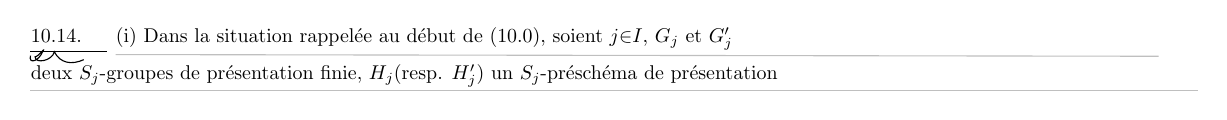
\begin{tikzpicture}[scale=.72,transform shape]
\node[anchor=base west,inner sep=0pt] at (0,0) {10.14.};
\node[anchor=base west,inner sep=0pt] at (1.5,0) {(i) Dans la situation rappelée au début de (10.0), soient $j\handwritten{\in}I$, $G_j$ et $G'_j$};
\node[anchor=base west,inner sep=0pt] at (0,-.65) {deux $S_j$-groupes de présentation finie, $H_j$(resp. $H'_j$) un $S_j$-préschéma de présentation};
\handwritten{\draw (0,-.16)--(1.35,-.16);
\draw (0,-.23) .. controls (-.04,-.38) and (.14,-.34) .. (.22,-.15) .. controls (.27,-.06) and (.14,-.25) .. (.08,-.25) .. controls (.08,-.38) and (.39,-.32) .. (.42,-.16) .. controls (.52,-.36) and (.72,-.40) .. (.94,-.30);
\draw[opacity=.25] (1.5,-.21)--(19.9,-.24);
\draw[opacity=.25] (0,-.85)--(20.6,-.85);}
\end{tikzpicture}}
